\documentclass[onlytextwidth]{beamer}
\usepackage[utf8]{inputenc}
\usepackage{microtype}
\usepackage{amsmath}
\usepackage{amssymb}
\usepackage[nomessages]{fp} %\FPeval{\var-name}{2*sin(pi/6)}
\usepackage{siunitx} %units in math. eg 20\milli\meter
\usepackage{yhmath} % for arcs, overparenth command
\usepackage{tikz} %graphics
\usetikzlibrary{quotes, angles}
%\usepackage{graphicx} already loaded by beamer class
%consider setting \graphicspath{{images/}}
%\parskip ?? to avoid paragraph indent
\usepackage{multicol} %may not need this package, just columns environment
\usepackage{venndiagram}

\subtitle[BECA]{Bronx Early College Academy}
\author[Huson]{Christopher J. Huson PhD}

\setbeamertemplate{headline}{\vskip2mm 
  BECA / \insertshortauthor \, / \inserttitle
  \hfill 
  \insertsection
  }

\title{Geometry Unit 1: Extra slides for Segments, Length, and Area}
\date{8-23 September 2022}

\begin{document}
\frame{\titlepage}

\section[Outline]{}
\frame{\tableofcontents}

\section{Extra 1.1 Segment addition }
\begin{frame}{Segment addition with fractions}

  \begin{block}{Do Now: Given $\overline{RST}$, $RS=3 \frac{2}{3}$, and $RT=9 \frac{1}{3}$. Find ${ST}$.}\vspace{0.5cm}
      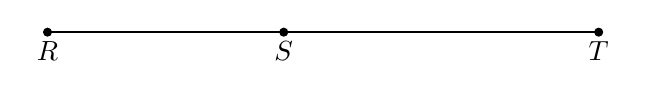
\begin{tikzpicture}
        \draw [-, thick] (0,0)--(7,0);
        \draw [fill] (0,0) circle [radius=0.05] node[below]{$R$};
        \draw [fill] (3,0) circle [radius=0.05] node[below]{$S$};
        \draw [fill] (7,0) circle [radius=0.05] node[below]{$T$};
      \end{tikzpicture}
  \end{block} \vspace{0.5cm}
\end{frame}

\begin{frame}{Mark the diagram and state your answer as a fraction}
    Given $\overline{RST}$, $RS=3 \frac{2}{3}$, and $RT=9 \frac{1}{3}$. Find ${ST}$.\\[0.75cm]
      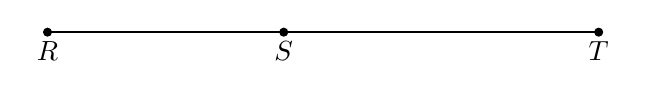
\begin{tikzpicture}
        \draw [-, thick] (0,0)--(7,0);
        \draw [fill] (0,0) circle [radius=0.05] node[below]{$R$};
        \draw [fill] (3,0) circle [radius=0.05] node[below]{$S$};
        \draw [fill] (7,0) circle [radius=0.05] node[below]{$T$};
      \end{tikzpicture} \\
      Solution \vspace{5cm} 
    \end{frame}
 

    \begin{frame}{Apply the Segment Addition Postulate \\
      Show your work by marking the diagram and writing an equation.}
        Given $\overline{DEF}$, $DE=8.5$, and $EF=2.5$. Find ${DF}$.\\[0.75cm]
          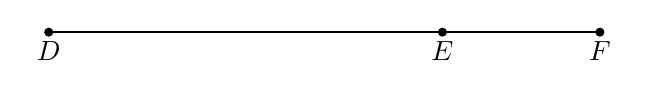
\begin{tikzpicture}
            \draw [-, thick] (0,0)--(7,0);
            \draw [fill] (0,0) circle [radius=0.05] node[below]{$D$};
            \draw [fill] (5,0) circle [radius=0.05] node[below]{$E$};
            \draw [fill] (7,0) circle [radius=0.05] node[below]{$F$};
          \end{tikzpicture} \vspace{4cm}
        \end{frame}
    
    \begin{frame}{Find the length of the line segment $\overline{PQ}$.}
      Given $P(-2)$ and $Q(3)$, as shown on the number line. \\[0.25cm]
        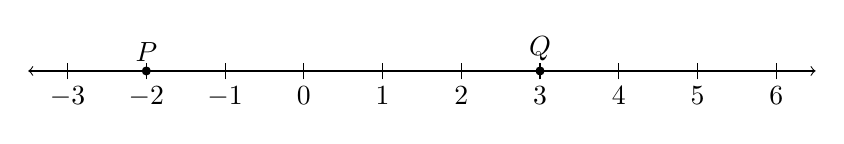
\begin{tikzpicture}
          \draw [<->] (-3.5,0)--(6.5,0);
          \draw [-, thick] (-2,0)--(3,0);
          \foreach \x in {-3,...,6} %2 leading for diff!=1
            \draw[shift={(\x,0)},color=black] (0pt,-3pt) -- (0pt,3pt) node[below=5pt]  {$\x$};
            \draw [fill] (-2,0) circle [radius=0.05] node[above] {$P$};
            \draw [fill] (3,0) circle [radius=0.05] node[above] {$Q$};
        \end{tikzpicture} \\
        State an equation and the solution. \\
    Check your work by counting the distance. Leave marks to show your work. \vspace{5cm}  
    \end{frame}
    
    \begin{frame}{Segment addition practice}
      \begin{block}{Do Now: Given $\overline{LMN}$, $LM=3x+1$, $MN=7$, $LN=17$. Find ${x}$.}
        \begin{tikzpicture}
          \draw [-, thick] (0,0)--(7,0);
          \draw [fill] (0,0) circle [radius=0.05] node[below]{$L$};
          \draw [fill] (4,0) circle [radius=0.05] node[below]{$M$};
          \draw [fill] (7,0) circle [radius=0.05] node[below]{$N$};
          \node at (1.7,0) [above]{$3x+1$};
          \node at (5.5,0) [above]{$7$};
          \draw [<->, dashed] (0,-1)--(7,-1);
          \node at (3.5,-1) [below]{$17$};
        \end{tikzpicture} 
      \begin{enumerate}
        \item Write down an equation to represent the situation.
        \item Solve for $x$.
        \item Check your answer.
      \end{enumerate}
      \end{block}
    \end{frame}
    
\begin{frame}{Midpoint example}
  \begin{block}{Given $M$ bisects $\overline{AB}$, $AM=5x+2$, $MB=20$.}
    \begin{enumerate}
      \item Mark the diagram with the values and tick marks
      \item Write an equation and solve for $x$
      \item Check your result
    \end{enumerate} \vspace{1cm}
      \begin{center}
        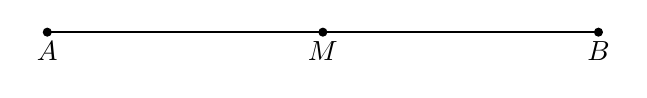
\begin{tikzpicture}
          \draw [fill] (0,0) circle [radius=0.05] node[below]{$A$};
          \draw [-, thick] (0,0)--(7,0);
          \draw [fill] (3.5,0) circle [radius=0.05] node[below]{$M$};
          \draw [fill] (7,0) circle [radius=0.05] node[below]{$B$};
          %\node at (1.7,0.5) [above]{$x+2$};
          %\node at (5.2,0.5) [above]{$11$};
          %\draw [<->, dashed] (0,-1)--(7,-1);
          %\node at (3.5,-1) [below]{$20$};
        \end{tikzpicture}
      \end{center}
  \end{block}
\end{frame}

\begin{frame}{Solve for $x$ given a bisector}
  Given $M$ is the midpoint of $\overline{AB}$, $AM=5x+2$, $MB=20$.
  \begin{enumerate}
    \item Mark the diagram with the values and tick marks
    \item Write an equation and solve for $x$
    \item Check your result
  \end{enumerate} \vspace{1cm}
    \begin{center}
      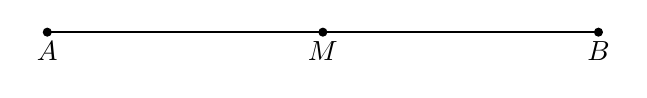
\begin{tikzpicture}
        \draw [fill] (0,0) circle [radius=0.05] node[below]{$A$};
        \draw [-, thick] (0,0)--(7,0);
        \draw [fill] (3.5,0) circle [radius=0.05] node[below]{$M$};
        \draw [fill] (7,0) circle [radius=0.05] node[below]{$B$};
        %\node at (1.7,0.5) [above]{$x+2$};
        %\node at (5.2,0.5) [above]{$11$};
        %\draw [<->, dashed] (0,-1)--(7,-1);
        %\node at (3.5,-1) [below]{$20$};
      \end{tikzpicture}
    \end{center} \vspace{4cm}
  \end{frame}
  
\begin{frame}{Segment bisector example}
  \begin{block}{Given $M$ bisects $\overline{PQ}$, $PM=x+7$, $PQ=23$.}
    \begin{enumerate}
      \item Mark the diagram with the values and tick marks
      \item Write an equation and solve for $x$
      \item Check your result
    \end{enumerate} \vspace{0.5cm}
      \begin{center}
        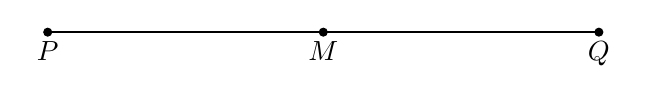
\begin{tikzpicture}
          \draw [fill] (0,0) circle [radius=0.05] node[below]{$P$};
          \draw [-, thick] (0,0)--(7,0);
          \draw [fill] (3.5,0) circle [radius=0.05] node[below]{$M$};
          \draw [fill] (7,0) circle [radius=0.05] node[below]{$Q$};
        \end{tikzpicture}
      \end{center}
  \end{block}
\end{frame}

\begin{frame}{Fraction and negatives+decimals practice problems}
  \begin{enumerate}
  \item Do Now: Given $\overline{DEFG}$, $DE=3 \frac{1}{4}$, $EF=6 \frac{1}{4}$, and $FG= 1 \frac{3}{4}$. (diagram not to scale)\\ [0.25cm]
    Find ${DG}$, expressed as a fraction, not a decimal.
    \begin{flushleft}
        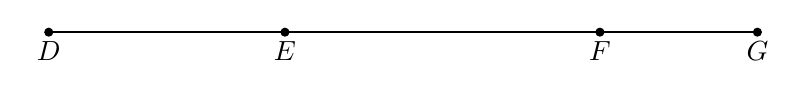
\begin{tikzpicture}
          \draw [-, thick] (0,0)--(9,0);
          \draw [fill] (0,0) circle [radius=0.05] node[below]{$D$};
          \draw [fill] (3,0) circle [radius=0.05] node[below]{$E$};
          \draw [fill] (7,0) circle [radius=0.05] node[below]{$F$};
          \draw [fill] (9,0) circle [radius=0.05] node[below]{$G$};
        \end{tikzpicture}
      \end{flushleft}
    
    \item Given $P(-2.4)$ and $Q(1.8)$, as shown on the number line. 
    Find the length of the line segment $\overline{PQ}$. 
    \begin{flushright}
      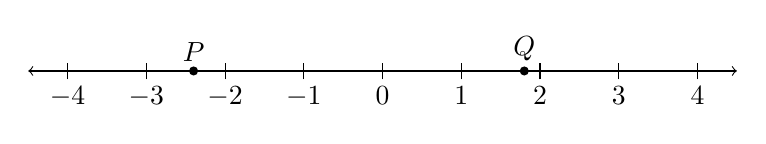
\begin{tikzpicture}
        \draw [<->] (-4.5,0)--(4.5,0);
        \draw [-, thick] (-2.4,0)--(1.8,0);
        \foreach \x in {-4,...,4} %2 leading for diff!=1
          \draw[shift={(\x,0)},color=black] (0pt,-3pt) -- (0pt,3pt) node[below=5pt]  {$\x$};
          \draw [fill] (-2.4,0) circle [radius=0.05] node[above] {$P$};
          \draw [fill] (1.8,0) circle [radius=0.05] node[above] {$Q$};
      \end{tikzpicture}
    \end{flushright}
    \end{enumerate}
  \end{frame}

\section{Sandbox}
\begin{frame}{Sandbox}
  \begin{enumerate}[(i)]
    \item one
    \item two
    \item three
  \end{enumerate}

  \fbox{box goes here \qquad xx \hspace{2cm} yy}

  \begin{enumerate}[T \quad F \,]
    \item one
    \item two
    \item three
  \end{enumerate}

  \begin{description}
    \item[End point] The point at the end of a line segments
    \item[Line] An infinite number of points extending in both directions forever 
  \end{description}

  \begin{definition}
    A \alert{prime number} is a number that has exactly two divisors. 
  \end{definition}
\end{frame}

\end{document}